\chapter{Interfaces}
\label{ch:SelectedDetails}

This Chapter describes an RDM-centric view of the organizations, software, services and facilities
with which RDM will interact.  These include the Mu2e TDAQ system,
the computer center and the follow-on data processing workflows.

\section{The Mu2e Online System}
\label{sec:Mu2eOnlineSystem}

This section briefly describes the elements of the Mu2e Online system that the reader will encounter in later sections.

\begin{description}
\item[OTS DAQ] ``Off-The-Shelf DAQ''~\cite{MU2EOTSDAQ}: the software used to provide configuration and top level run-time control of the TDAQ system.
  Shifters will modify run configurations, start runs and stop runs using OTS DAQ.
\item[OTS DB] OTS DAQ stores its configurations in an instance of a MongoDB database.
  This is variously called the ``OTS database'' or the ``Mongo database''.
  This database may also be used to store run summary information.
  It may also be used to store conditions data for use by online processes;
  if it is used for this purpose, it is also the online conditions DB.
\item[\artdaq] The software used to control processes and to move data between processes on the TDAQ Servers and the TDAQ Data Logger machines.
\item[DCS] ``Detector Control System''.
  For details see~\cite{DCSSpec};
  this is also known as the ``slow control system'' or the ``EPICS system''
  Its functions include:
  \begin{enumerate}
    \item Set hardware configurations and limits, for example, voltages.  Turn hardware on and off.
    \item Read back and store process variables (PV) such as voltages, currents, temperatures, heartbeats etc.
    \item Monitor PVs: alarm if out of tolerance; display timelines on request.
  \end{enumerate}
\item[EPICS] The name of software technology used to implement the DCS.
\item[EPICS DB] EPICS stores its PV+timestamp data in a relational database.
  This is often called the ``EPICS DB'' but this is a misnomer because it will likely use
  a general purpose relational database that will be used by EPICS
  and by other online software.
\end{description}
Both OTS DAQ and \artdaq are developed and supported by the Fermilab SCD;
they are used by Mu2e and by other experiments. EPICS is widely use for slow
control by other experiments at Fermilab.


\section{Block Diagram}
\label{sec:BlockDiagram}

Figure~\ref{fig:blockdiagram} shows a block diagram of the major elements involved
in the data flow from the experiment hardware to long term storage; it also shows
some of the elements of the offline data processing.
All elements in the left hand dot-dashed box are located in the Mu2e Hall
and, except for the Mu2e building router, are the responsibility of the various Mu2e groups.
All elements in the middle dot-dashed box are located in the computer center
and are the responsibility of SCD; the internal details of the SCD-managed resources
are not shown and the RDM will treat these resources as a interconnected, coherent whole.
The Mu2e building router and the optical fiber that connects that router
to the computer center are the responsibility of CCD;
see Appendix~\ref{app:RouterAndNetwork} for details.
The right hand dot-dashed box names some of Mu2e Offline data processing workflows
that will read data from storage in the computer center, process it,
and write data back to storage computer center.
The first workflow in this chain is Pass1, which will run soon after new files
are resident on storage in the computer center and are registered in the file catalog;
for additional details of the offline data processing workflows see Section~\ref{sec:downstreamProcessing}.

\begin{figure}[tbp]
\centering
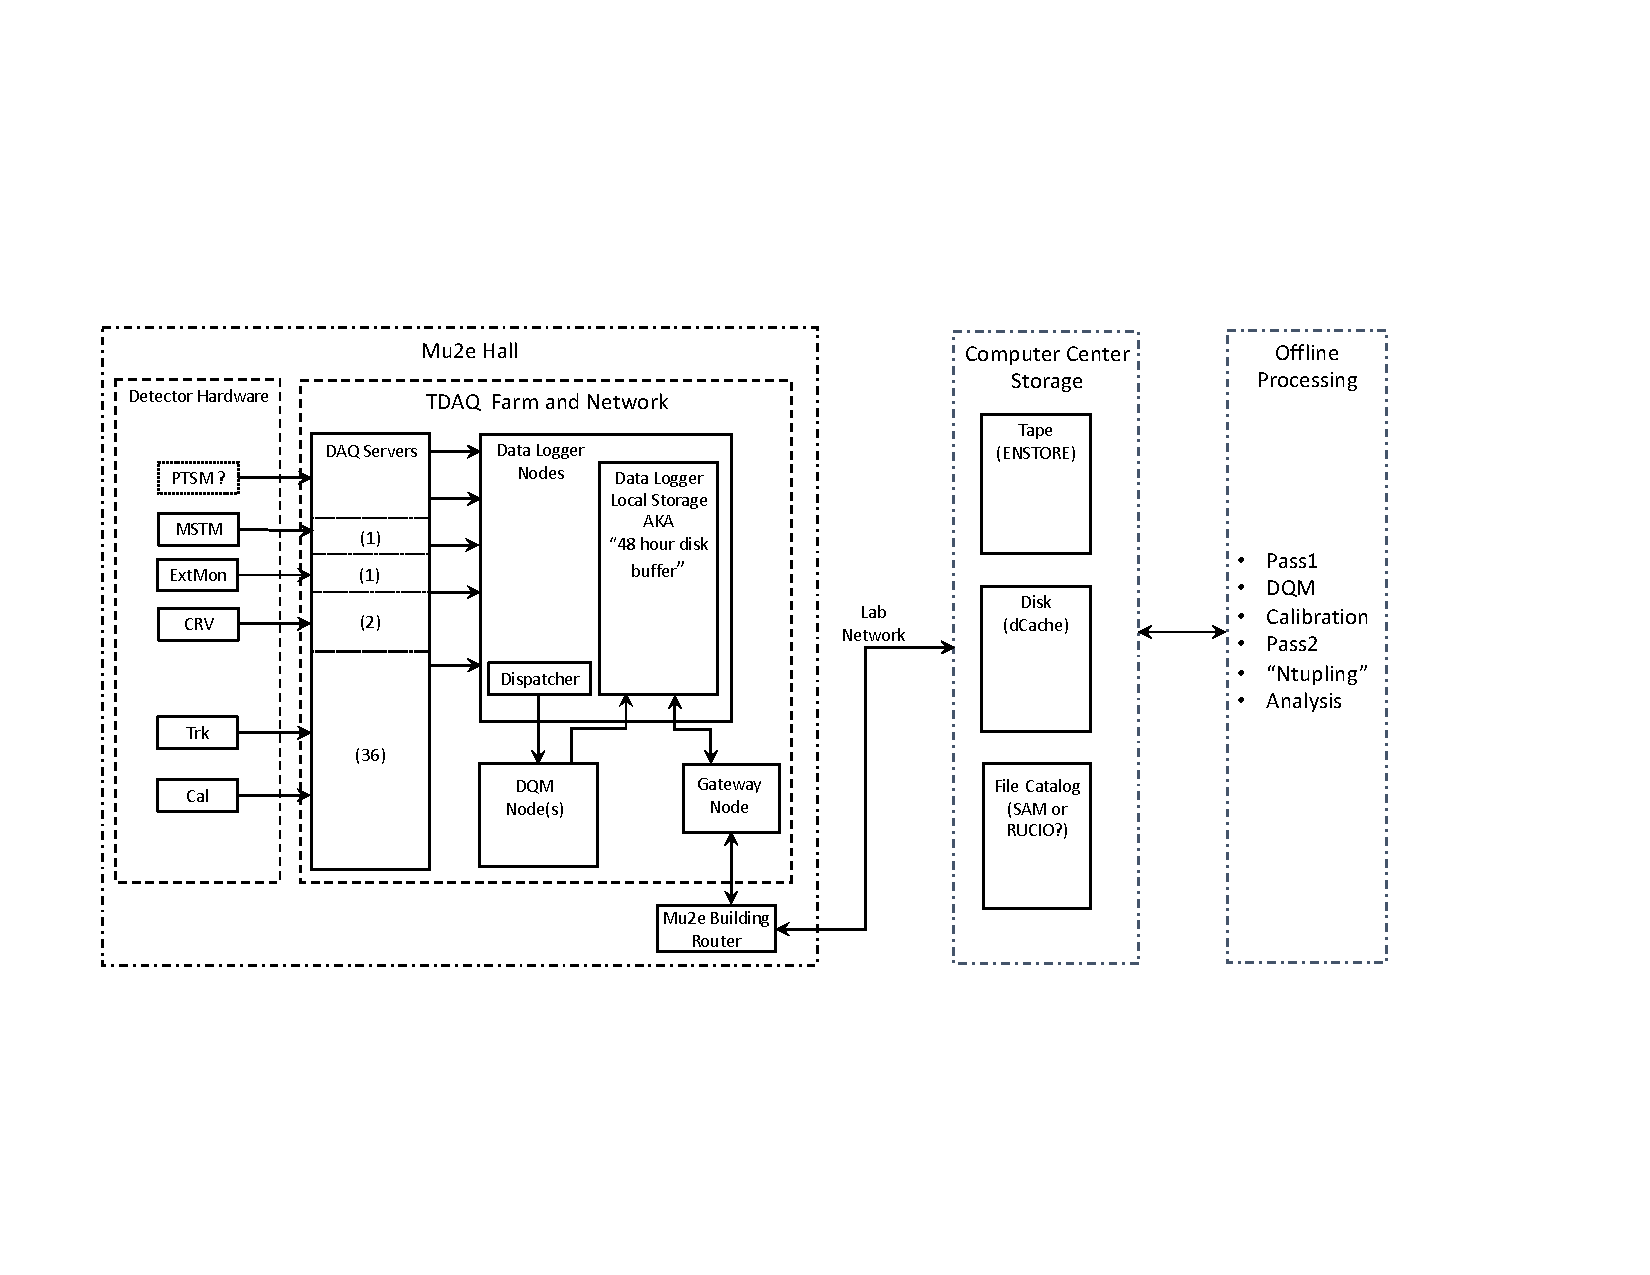
\includegraphics[width=0.9\textwidth]{figures/interface_with_TDAQ.pdf}
\caption[Block diagram of interfaces seen by the Mu2e RDM]{
  Block diagram of the world seen by the Mu2e RDM.
  See the text for a discussion of these elements.}
\label{fig:blockdiagram}
\end{figure}

Data flows from the detectors, through the readout electronics,
through the DAQ system and into the TDAQ computer farm.
The five approved detectors are the Tracker (Trk), Calorimeter (Cal), the Cosmic Ray Veto system (CRV),
the Muon Stopping Target Monitor (MSTM) and the downstream Extinction Monitor (ExtMon).
A sixth detector has been proposed, the Production Target Scanning Monitor (PTSM),
which is drawn with a dotted box;
it's primary use is to send rapid feedback to the accelerator control room
and it's not clear what, if any, data it will send through the TDAQ system.
It is only mentioned here for completeness;
the data volume, if any, from the PTSM will be small enough that it will not be
a driver for the RDM.

A cartoon picture of the TDAQ computer farm is that it has 40 DAQ Server nodes
that talk to the detector electronics, build events and run trigger algorithms on those events.
The design is a dead-timeless streaming DAQ system that has no hardware trigger;
it reads every event from the detector hardware and sends all events to software filters
that run on the DAQ server nodes;
the software makes the trigger decision.
The present design is 20 software filter processes on each of the 40 DAQ server nodes, 800 total.
Events that pass the trigger are forwarded to Data Logger nodes that will write the events
to files in the Data Logger Local Storage (DLLS), a RAID 0 hybrid SSD/HDD array on the bus of the Data Logger nodes.
Appendix~\ref{app:DataLoggerLocalStorage} has the specs for and a discussion about the DLLS.
In earlier DPC related talks and documents the DLLS  was referred to as the ``48 hour disk buffer''.
In addition to the events that trigger because they are interesting,
a several prescaled samples of the remaining events will pass the
trigger and will be handled the same as the interesting events.
Finally, there will be special data streams for calibrations.

The base design is to have a two data logger nodes that receive the data from all DAQ server nodes
and write it to files in the DLLS.
The data logger nodes will write several files, each containing events selected by a different algorithm.
Details can be found in Chapters~\ref{ch:DataStreamsAndFileStreams} through~\ref{ch:file_streams}.

The Data Logger nodes will also host a process called a ``Dispatcher''
that requests events from the DAQ and forwards them to clients.
The Dispatcher is designed to exert no back pressure on the DAQ
and, therefore, will normally see only a subset of the events.
Two of the clients foreseen for the Dispatcher are an Event Display and
a Data Quality Monitoring (DQM) system,
which will produce histograms, timelines etc that can be viewed in real time.
Periodically the DQM system will write its histograms, log files etc to
files in the data logger local storage.  One of the jobs of the RDM will be
to move these files to long term storage.

All of the computing resources in the TDAQ farm are on a private subnet
that cannot been seen from the lab network.  Access in and out
of the private subnet will be via a gateway node that is connected to
both the private subnet and the lab network.
Purchasing and maintaining the gateway node is the responsibility of the TDAQ group.

When the Mu2e Hall was built and provisioned, CCD personnel installed a dual router
and connected it to the lab optical fiber network.
RDM will move data from the Mu2e Hall
to the computer center using this router and the lab optical fiber network.
The router is a standard item that CCD uses in many places and it stocks spares.
CCD is responsible for the maintenance of both the router and the network.
See Appendix~\ref{app:RouterAndNetwork} for the
specs of this router and for details of the arrangement with with CCD,
including costs that must be paid by Mu2e to CCD for this service.


For the foreseeable future Mu2e expects that the disk and tape services provided
by SCD will be dCache and ENSTORE.
At this writing Mu2e is using SAM as the file catalog system for files produced
by simulations, tests stands and Vertical Slice Tests (VST).
SCD plans to phase out SAM and replace it with a more modern system, RUCIO\cite{RUCIOHome};
RUCIO is already in use by CMS and by DUNE for Proto-DUNE Single Phase data.
It is almost certain that SAM will be phased out during the lifetime of Mu2e.
One of the questions to ask in the design of the RDM is
when to make the transition to RUCIO.

\section{The EventWindowTag and the EventMode}
\label{sec:EWTagAndEventMode}

The heart of the TDAQ system is the Command Fan-Out (CFO), an FPGA that delivers
configuration information and timing signals to all elements of the DAQ.
The inputs to the CFO are the RF0 signal from the accelerator
and a Run Plan that comes from OTS DAQ.
Just prior to the start of each event,
the CFO distributes a 16-byte heartbeat packet that describes the upcoming event~\cite{PacketProtocols};
among other things, this contains the EventWindowTag (EWT) and EventMode fields,
both of which will be discussed below.

An event window is defined as time interval during which the DAQ collects data for one event.
Each event window is identified by a 48 bit integer field in the heartbeat packet, called
the Event Window Tag (EWT);
the EWT will be monotonically increasing throughout the Mu2e experiment and
enough bits have been reserved for it to produce unique identifiers for all
events over a many-year run.
The CFO is responsible for incrementing the EWT and putting the correct value into
the heartbeat packet for each event.
The detector readout electronics label information from their subsystem with the EWT.
The event builders use the EWT as the key for event building.

The Mu2e detector can operate in many modes, two of which,
on-spill and off-spill, will be discussed in the next section.
In addition there will be many calibration modes.
All elements of the TDAQ have pre-programmed operations defined for each mode.
When the CFO creates the heartbeat packet for each event,
it sets a 4 byte EventMode (EM) field
that tells the TDAQ system in which mode to operate for the upcoming event.

\section{On-Spill, Off-Spill and Near-Spill}

This section defines the concepts of on-spill, off-spill and near-spill running.

It is expected that, for most of it's running time,
Mu2e will share the Fermilab Main Injector with a neutrino experiment,
first, with NOvA and, later, with DUNE.
To keep this document easier to read it will discuss sharing with NOvA but sharing with DUNE is implied.
The change from NOvA to DUNE may change details
but will not materially change the requirements of the RDM.

Sharing with NOvA drives the repeating cycle of Mu2e operations, a Main Injector (MI) cycle of
21 Booster (BO) cycles.
The duration of one Booster cycle is 1/15~s,
making the duration of one MI cycle 1.4~s.
Figure~\ref{fig:beamMacroStructure} shows a cartoon of the MI cycle.
From the Mu2e point of view, the cycle starts with a series of 8 slow spills
from the Delivery Ring (DR) to the Mu2e production target;
within each spill, proton pulses arrive at Mu2e every 1695~ns;
the duration of a spill is nominally 25,438 pulses, about 43.1~ms.
There is a gap of about 5~ms between spills.
The eighth spill is followed by a period of about 1020~ms,
during which no proton pulses arrive at Mu2e;
during this time, beam is delivered to NOvA
and beam is prepared for the next 8 spills to Mu2e.
Then the cycle repeats.

\begin{figure}[tbp]
\centering
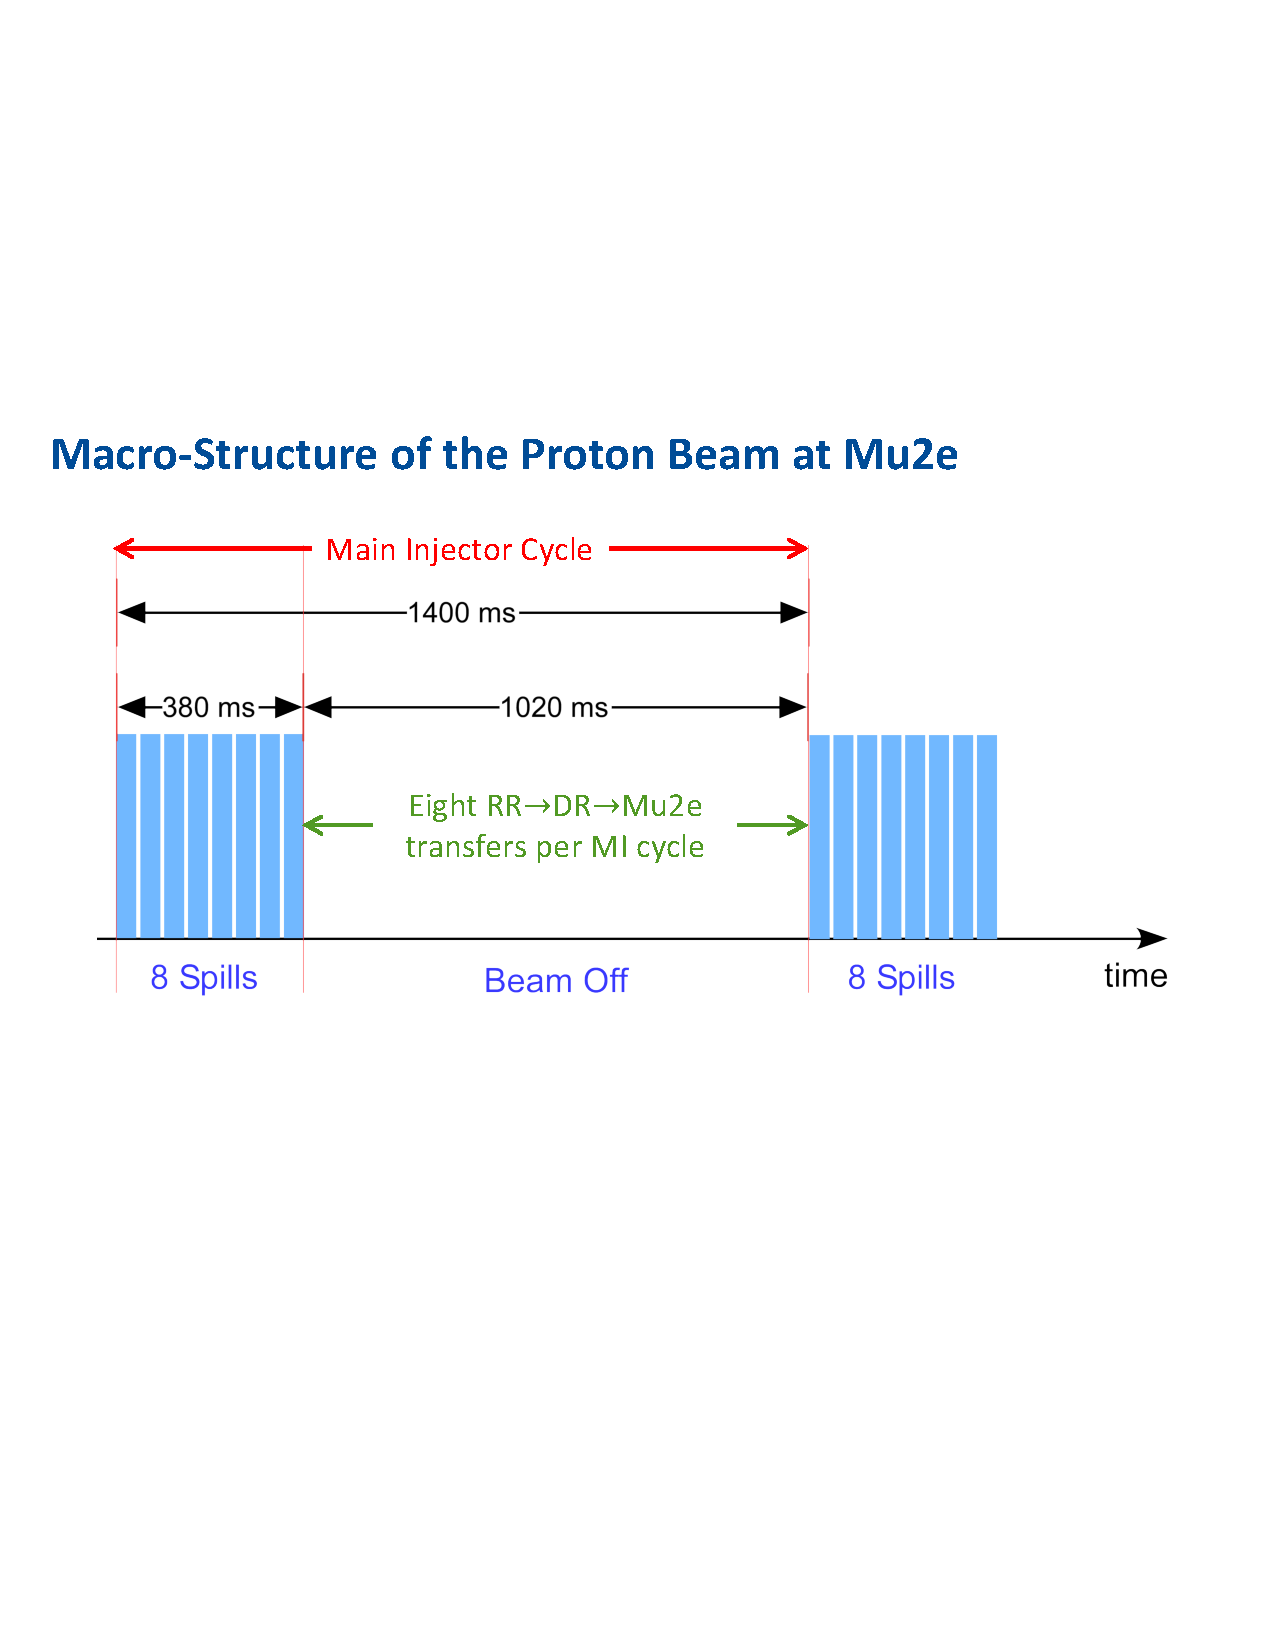
\includegraphics[width=0.9\textwidth]{figures/ProtonBeamLongitudinalStructure2019-01-10_page6.pdf}
\caption[Macro Structure of the Proton Beam at Mu2e]{
  Macro Structure of the proton beam at Mu2e, taken from page~6 of
  the file ``Proton Beam Longitudinal Structure (.pdf)'' from
  Reference~\protect{\cite{beamTiming}}.  The figure is described in the text.}
\label{fig:beamMacroStructure}
\end{figure}

During the spills, Mu2e is running in the on-spill configuration.
During the 1020~ms no-beam period, Mu2e is running in the off-spill configuration.
It has not yet been decided if the 5~ms periods between spills will
be in the on-spill or off-spill configuration
but that does not materially affect the design of the RDM.
Table~\ref{tab:timescales} summarizes the time scales within one MI cycle.
\begin{table}
\begin{center}
\caption[Properties of the Beam-to-Mu2e MI Cycle]{Properties of Beam-to-Mu2e MI Cycle.}
\label{tab:timescales}
\begin{tabular}{ll}\hline
   1/15~s & Period of one Booster cycle \\
   21     & Booster cycles in one MI cycle \\
   1.4~s  & Period of one MI cycle \\
   43.1~ms & Duration of one spill \\
   8       & Number of spills per MI cycle \\
    5~ms   & Duration of the period between two spills \\
   1020~ms & Duration of the off-spill period within one MI cycle \\
   1695~ns & Period of the Delivery Ring and the duration of one on-spill event\\
   100~$\mu$s & Duration of one off-spill event \\
   24.6\%     & Duty factor (total spill time divided by MI cycle duration)\\
   \hline
  \end{tabular}
\end{center}
\end{table}


In the on-spill configuration, one event will have  a duration of 1695~ns
and it records the information associated with one proton pulse.
The trigger will be configured to select interesting events associated with the proton pulse
and to prescale other events in order to study the performance of the trigger.
In the off-spill configuration, one event will have a duration of 100~$\mu$s.
During the off-spill period, Mu2e will trigger on cosmic rays that
pass through the tracker and/or the calorimeter; it will also collect
pedestal data from some of the subsystems; some calibration procedures
may also take place during the off-spill period.

Mu2e expects that the accelerator super-cycle will consist of a
sequence of many of the above MI cycles,
with an occasional other cycle mixed in.
For example, when MTEST is active, there is usually beam delivered to MTEST about once per minute.
When this occurs, Mu2e will have an additional few seconds off-spill running.

There will also be periods in which the accelerator complex is not delivering
beam to Mu2e for an extended time, minutes, hours, days or weeks.
In some of these periods Mu2e will shutdown to perform maintenance, repairs or upgrades;
in others Mu2e will execute calibration runs;
and in others Mu2e will collect data in off-spill mode for an extended period of time.


The Mu2e TDAQ team have defined a value of the Event Mode that they have named near-spill.
This is to allow for the possibility that some subsystems may want to
configure themselves differently during the transition from on-spill to off-spill.
At this time there are no definite plans to use this mode but it is available if needed.

The design of the Mu2e TDAQ system is that trigger processing lags the incoming events
during the on-spill period and catches up during the off-spill period.  There is
buffering distributed throughout the TDAQ system to support this.

It's possible that the MI cycle might need to be increased to 22 Booster cycles to
allow for hysteresis in the MI electromagnets;
should that happen, the additional time will be allocated to a longer off-spill period.
This does not significantly change the requirements for the RDM.

Mu2e plans to start operations with a slightly different configuration:
4 spills instead of 8, where each spill has a longer duration than 43.1~ms;
this mode is called ``one batch'' running or ``Phase~1'' running;
the 8 spill configuration is called ``two batch'' running or ``Phase~2'' running.
The data volume produced in one batch running will be about 60\% of that produced
in two batch running; otherwise the requirements for the two are the same.

There will be times when Mu2e is taking data but NOvA is not.
In such times, the base plan is that Mu2e will continue to take data using the same MI cycle of 21 Booster cycles.
There are several technical limitations that prevent Mu2e from reducing the off-spill period
in order to increase the duty factor:
there are radiation safety limits on the average beam power;
the production target will have a reduced lifetime at higher average beam power;
the TDAQ system cannot accommodate a significantly higher event rate because it
uses the off-spill period to catch up on buffered events.

\fixme{Is the following correct: these limitations have some headroom during one batch running;
  so we could see a shorter MI cycle during one batch running.}

\section{EventIDs, Runs and Subruns}
\label{sec:TagsIDsRunsSubRuns}


Mu2e uses the \art event processing framework;
the trigger filter processes that run in the trigger farm will each be a separate \art process;
the {\code artdaq::DataLogger} processes will each be \art processes;
\art will also be used for offline data processing.
In \art, events are uniquely identified by a 3 part identifier called an
{\code art::EventID}; the parts are named run number, subrun number
and event number.

Within the DAQ system, event fragments and fully assembled events
are identified by their Event Window Tag (EWT).
The DAQ system will translate each EWT to an {\code art::EventID}
before events are presented to the \art based software filter processes~\cite{EventLabels}.
The mapping of EWT to  {\code art::EventID} will be unique and
{\code art::EventID}'s will be monotonically increasing with the time
that the event occurred.
The EWT will be recorded as part of the \art data for each event.

The ExtMon and MSTM teams have discussed writing some or all of their data in non-\art formats
in which the data is identified by an EWT, not an {\code art::EventID}.
The information needed to convert between these two representations
will be available in the offline environment.
This will allow correlating ExtMon and MSTM data with the data stored in \art format.

The meaning of run and subrun are defined by Mu2e.
All that \art requires is that a subrun contain zero or more
events and that a run contain zero or more subruns.

The current plan is that runs will typically have a duration of a few hours
while subruns will contain an integer number of MI cycles and
have a duration somewhere between 14 seconds and a few minutes.
This means that each subrun will contain both on-spill and
off-spill events.
The transition between subruns will happen during the off-spill period,
which ensures that each on-spill period is contained within a single subrun.

These durations are informed by the following.
Mu2e has designed a conditions management system
in which intervals of validity (IOV) are a specified as a range of subruns;
such a range may either span runs or be contained within a single run.
Therefore subruns must be short enough to follow the most
rapidly changing conditions.  As of this writing it seems
likely that the upper limit for the duration of a subrun will
be driven by considerations of data handling and downstream data processing;
that is, files should be neither too big nor too small for efficient data handling
and Pass1 jobs should be able to process one subrun in, at most, a few hours.

The Mu2e TDAQ has been designed so that subrun transitions will be deadtimeless
but that data taking will pause for a few minutes at run transitions.
At each run transition the TDAQ system will do some house keeping,
including resetting some hardware, reloading some firmware and restarting some processes.
These steps are designed to cure any Single Event Upsets (SEU) in the firmware
and to cure any configuration drift or system lockup.
Therefore a run should be long enough that the dead time
caused by the run transition is a small fraction of the total run time
but short enough that the resets occur frequently enough
to keep the system robust.

Anomalies that occur during data taking will cause some runs
and subruns to be cut short.
Therefore the RDM must expect some files that are smaller than normal
and even empty files.


\section{Organization of Data by Detector Subsystem }
\label{ssec:dataOrganization}

This section will give an outline of how data from the
various detector subsystems flows from the detector to the DLLS.
This will help explain why the data organization in the DLLS is what it is.
The text in this section refers to Figure~\ref{fig:filesDLLS}.
These descriptions are only high level overviews,
intended to convey enough background information to design the RMD.

\fixme{References to the full TDAQ docs.}

\begin{figure}[tbp]
\centering
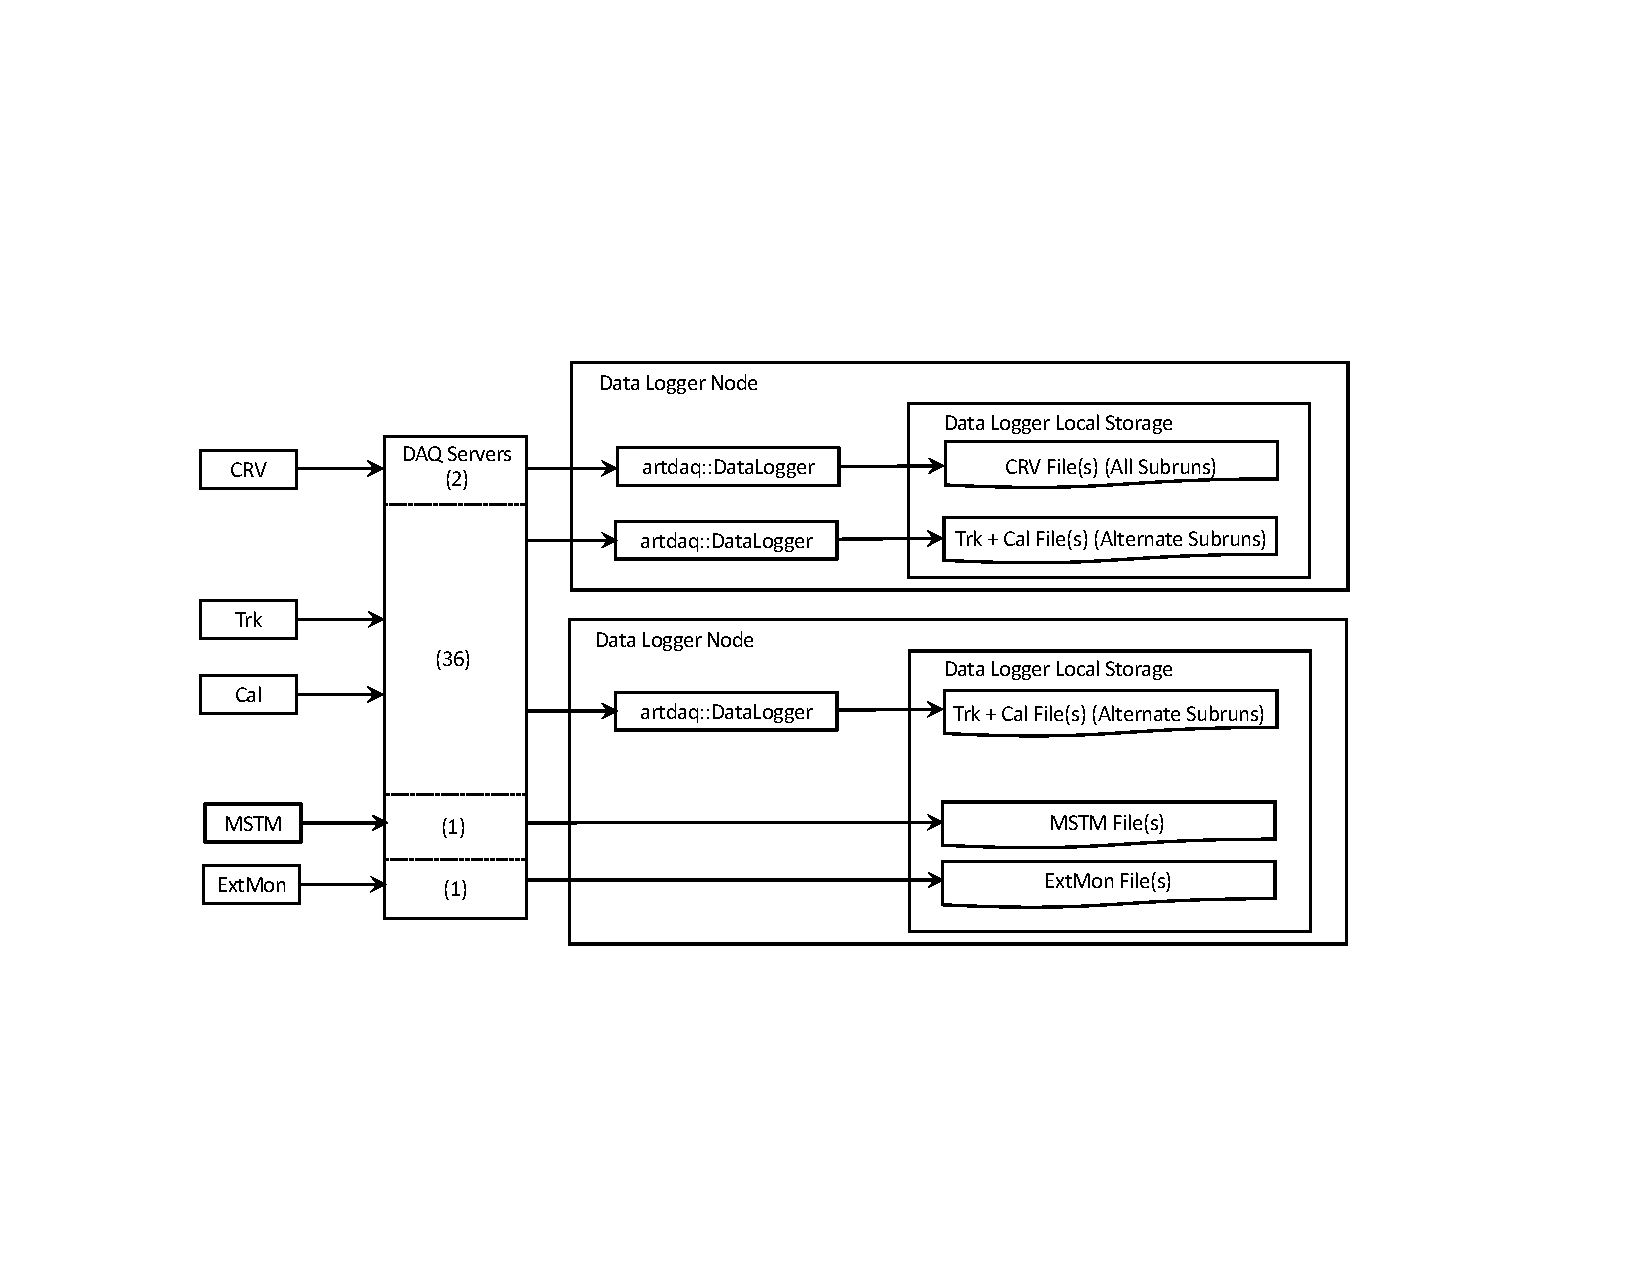
\includegraphics[width=0.9\textwidth]{figures/FilesInDLLS.pdf}
\caption[Files in the DLLS]{
  Files in the Data Logger Local Store; the figure is described in the text.}
\label{fig:filesDLLS}
\end{figure}


\subsection{Tracker and Calorimeter}
\label{ssec:TrkAndCal}

Data flows from the tracker and calorimeter into FPGAs mounted on the PCIe bus of 36 of the 40 DAQ servers;
these FPGAs are called Data Transfer Controllers (DTC).
All DTCs on these 36 DAQ servers communicate with each other over a high speed switch
and perform event building.
Event building uses only resources on the DTCs and is independent of operations on the host DAQ servers.
The end product of event building is that each DTC contains buffers of complete events held in its own memory;
each event is complete in the sense that it contains all of the data from the tracker and calorimeter
but it does not contain any data from other subsystems.
Every event is present in exactly one buffer and each DTC sees only a small subset of the full event stream.

Once a DTC has a full buffer of events it will transfer that buffer to its host DAQ server;
it does so by transferring it to an {\code artdaq::BoardReader} process.  On most of the
36 DAQ severs there are two DTCs and two {\code artdaq::BoardReader} processes;
on the remaining servers there is one DTC and one {\code artdaq::BoardReader} process.

The trigger filter processes on each DAQ Server are controlled by a process
called an {\code artdaq::EventBuilder}.
This name is historical and reflects the function that it had for earlier experiments in which \artdaq was developed.
For Mu2e, event building will be done in the DTCs and the function of an
{\code artdaq::EventBuilder} process is to receive events from
the {\code artdaq::BoardReader} processes and to distribute them to the trigger filter \art processes
that it controls.

If an {\code artdaq::EventBuilder} has trigger filter processes that are ready for their next event,
and if no events are available from any of the {\code artdaq::BoardReader} processes on that server,
then the {\code artdaq::EventBuilder} can fetch events from {\code artdaq::BoardReader} processes
on other DAQ servers.
This allows all 40 DAQ servers to run trigger filter processes even though only 36 of the 40 servers
communicate with the tracker and calorimeter.

The end result is that each event will be seen by exactly one of the trigger filter processes.
Within one trigger filter process there is no guarantee that events within one subrun will arrive in
increasing order of {\code art::EventID}.

\fixme{Is there a guarantee that, within a single process all events from subrun n will be seen before
  any events from subrun n+1?  If so, for personal interest, how is this guaranteed?
  I am thinking of a process running on, the CRV, ExtMon or MSTM servers; these get all of their
  events from BoardReaders on other machines.  I can see that they will usually be in increasing order
  but I don't see a requirement that they be in increasing order.
}

The trigger filters make a trigger decision on each event.
The current expectation is that about 1 in 400 events will pass the trigger;
this includes all events that pass the primary or support triggers
and prescaled events that fail at selected places during trigger processing;
random triggers are included in the last category.
Throughout this document the phrase ``passes the trigger'', without additional modifiers,
refers to all of the above.
The trigger rate is dominated by prescaled support triggers,
which are designed to select events for calibration and monitoring.
Details of the software trigger system, as of May 2021,
are available in reference~\cite{TriggerSU2020}.


Each \art trigger filter process sends events that pass the trigger over a network
to one of the two data logger nodes where they are received by an {\code artdaq::DataLogger} process
that writes the events to files in the DLLS.
This process may be configured to write all events to a single file
or to split the events across several files,
for example all on-spill events to one file and all off-spill events to another.
It has yet to be determined exactly how many files will be written
by each {\code artdaq::DataLogger}.

\begin{sloppypar}
Because different events have very different trigger processing times
and because {\code artdaq::EventBuilder} processes can draw events from
any of the {\code artdaq::BoardReader} processes, events will arrive at the
{\code artdaq::DataLogger} out of order.  In particular, early events from subrun N+1
may arrive at an {\code artdaq::DataLogger} before the last event from subrun N.
\end{sloppypar}

The TDAQ base design has two Data Logger nodes, each running an
{\code artdaq::DataLogger} process that will receive tracker and calorimeter events.
The plan is to send events from alternate subruns to each of the two.
This allows a clean separation of the event stream into non-overlapping subruns.
Within a each subrun, however, the events may not be in order.

\fixme{If we end up with short subruns, say 10 MI cycles, 14 s, will we need to stripe
  this 3 or 4 wide to survive the longest processing latencies?}

At the big picture level, the above story is the same for both on-spill and off-spill running.
There are two important differences in details.
First, the trigger filter processes test the EventMode
and run different algorithms for the two cases;
second, the rate of triggered events
and data volume per triggered event will be much smaller in off-spill events than in on-spill events.

The behavior for other event modes is not yet known.

\subsection{Cosmic Ray Veto}
\label{ssec:CRV}

This subsection also discusses Figure~\ref{fig:filesDLLS}.
In on-spill running,
data from the CRV system is read from the detectors and held in buffers in the
readout electronics chain.
When one of the trigger filter processes described in the previous section
decides that an event has triggered,
it sends a message to the CRV system and requests that information from that
event be forwarded to a Data Logger node.
The requested information flows from the readout electronics through 2 two of the 40 DAQ servers
to a third {\code artdaq::DataLogger} process that is running on one of the Data Logger nodes.
This third {\code artdaq::DataLogger} process writes the events to files in the DLLS.
Again, this process may be configured to write all events to a single file
or to split the events across several files,
perhaps on-spill events to one file and off-spill events to another.
The details are to be determined.

\fixme{where are the buffers? ROC? FEB?}

The end result is that each event in the DLLS will be split across two files, one with the
tracker and calorimeter data and one with the CRV data.
One of the questions to be answered when designing the RMD will be to identify
the point in the workflow that these two event fragments will be joined into a single file.
There are insufficient computing resources to do this step in the Mu2e online environment.
Therefore it will have to be done after data has been copied to the computer center.
One of the questions in designing the RDM will be to work with the Pass1 team to
decide if the responsibility for this job is part of the RDM or if it is part of Pass1.

\begin{sloppypar}
The original design of the TDAQ was the that an {\code artdaq::DataLogger} process
would receive the tracker and calorimeter information for triggered events
and buffer it internally until the CRV information arrived.
After the CRV information arrived,
the {\code artdaq::DataLogger} process would write an event containing information from all 3 subsystems.
As the TDAQ design matured, the TDAQ team became concerned that this scheme would not work because
of two factors could conspire to exceed the buffering capacity within the CRV readout electronics;
the factors are the tail to long processing times in the trigger filters
and the size of the CRV data.
Therefore this plan was replaced with that described above.
\end{sloppypar}

It is the strong preference of the DPC team that the decision to split the data
for one event into two files be revisited from time to time.
If new information indicates that the TDAQ team can revert to the original, non-split
configuration, we request that they do so.


The light sensors for the CRV system are Silicon Photo multipliers (SiPM).
The CRV team have requested that, during off-spill running,
TDAQ acquire as large a sample of untriggered SiPM data as is practical;
they will use this data to study the time dependence of the SiPM pedestals.
This data is sometimes called ``SiPM noise data'', ``SiPM pedestal data''
or ``SiPM pedestal events''.

Mu2e will automatically get a small sample of SiPM pedestal data from the off-spill events
that trigger based on tracker and calorimeter data.
However this trigger rate will be only of O(20 Hz), which will not yield enough SiPM pedestal data.
One option is for the trigger filters to prescale off-spill events that fail the trigger
and to do so at a rate that will produce a large enough sample of SiPM pedestal data.
In this case SiPM pedestal events will include information from the tracker and calorimeter as well,
albeit in separate files.
A second option is for an independent agent within the TDAQ system to trigger the SiPM pedestal events;
in this case SiPM pedestal events will not contain tracker and calorimeter information.
The TDAQ team has not yet decided between these options.

\fixme{If the collaboration has a preference, they should make it known. Do we need a section with
questions for the collaboration?}

\subsection{Extinction Monitor}
\label{ssec:ExtMon}

Data from the Extinction monitor will be read independently of data
from the tracker, calorimeter, CRV and MSTM.
Its path to the DLLS will also be independent, as is indicated in Figure~\ref{fig:filesDLLS}.

The Extinction Monitor has two subsystems, a pixel telescope and the Accelerator
Fast Feedback (AFF) monitor.
Both are located in a cavern to the side of the proton beam dump
and both view a collimated piece of the phase space of secondary particles produced by the interaction
of the proton beam in the production target.

The job of the pixel telescope is to count the number of tracks that it sees in-time with the proton pulse and the number
of tracks that it sees during the interval between proton pulses.
If everything is working well, the first number will be about 40 per proton pulse
and the second number will almost always be zero.
If the second number is non-zero more than once every few hours it indicates a problem with the accelerator.

\fixme{Is 40 per proton pulse the right number?  Check with Andrei/Matthew.}

The pixel telescope hardware will be read out by a computer that is located in the cavern.
This computer will process the raw data and send summary data plus
several types of prescaled raw and intermediate level data to one server in the DAQ Server farm.
The ExtMon Summary data will be available for the off-spill period for every event but,
due to bandwidth limitations in the pixel readout,
the on-spill summary data will only be available every N events, where N will be something like 10 or 20.
The server in the DAQ Server farm will receive the data and write it to one or more files in
the DLLS.

\fixme{Get a reference for the pixel telescope summary data.}

The AFF is a thick panel of scintillator that produces light when the secondary beam particles pass through it~\cite{ExtMonAFF}.
For each proton pulse, the system will measure the light produced in-time with the proton pulse,
which will be used as a proxy for the number of protons in the pulse.
This information, 128 bits per proton pulse,  will be sent to the accelerator control room to provide fast feedback
to regulate slow extraction.
A copy of this information will also be sent through the TDAQ to a file in the DLLS.
This system will also prescale raw and intermediate level data and send that through the
the DAQ Server to the DLLS.

The pixel telescope summary data and the AFF summary data  will both be small while the prescaled raw and intermediate
level data will be large.
It is likely that for each of the pixel telescope and the AFF, the summary data will be written to
one file in the DLLS while the other data will be written to one or more other files in the DLLS.

The details of the file formats have yet to be decided.
It has also not been decided if the data will be written to the DLLS
via an {\code artdaq::DataLogger} process
or by some other means.

\begin{sloppypar}
The DAQ Server assigned to the ExtMon will also run trigger filter processes that receive
data from {\code artdaq::BoardReader} processes on other DAQ servers.
\end{sloppypar}

\fixme{What are the downstream work flows for this data.  Likely the summary data from both subsystems
  will go into a database and retrieved from that db as needed by offline jobs.
  Probably it needs to be organized for retrieval by subrun?  Whose job is it to define the format?
  Where does RDM's job end - do we need to populate the db as well as putting the file on tape?
  Or is that Pass1?
}


\fixme{If the data does not flow through {\code artdaq::DataLogger} what will it be?
  Eric says no NSF mount on the DAQ servers because of reliability.  So something else?
  }

\subsection{Muon Stopping Target Monitor}
\label{ssec:MSTM}

The story of data from the MSTM is similar to that of data from the ExtMon.
Data from the MSTM  will be read independently of data
from the tracker, calorimeter, CRV and ExtMon.
Its path to the DLLS will also be independent, as is indicated in Figure~\ref{fig:filesDLLS}.

The MSTM consists of two scintillating crystals located behind collimators in a shielded area
at the far east end of the detector hall.
One crystal is High Precision Germanium (HPGe) while the other is Lanthanum Bromide (LaBr).
The crystals and collimators are aligned so that the crystals will see X-rays and gamma rays
produced in the Muon stopping target foils.
The process of muon capture on the stopping target foils to form a muonic atom
emits characteristic X-ray lines; these X-rays are prompt.
The process of muon capture from a bound state onto a nucleus produces
a variety of excited nuclei that decay by emission characteristic gamma ray lines;
some of these gamma rays are prompt and others have half lives of seconds to minutes.
The intensity of these lines is proportional to the number of stopped muons and therefore
to the denominator of $R_{\mu e}$, the main measurement of the Mu2e experiment.,
The MSTM detectors will measure the energy of each photon that it sees
and will accumulate an energy spectrum over a period of a few minutes.
The plan is to measure the intensity of the characteristic narrow lines in each spectrum and,
from that, infer the number of muons that have stopped in the stopping target during
that period.

The pulses produced by photons in these crystals will be measured by waveform digitizers that are read out
by computers located close to the crystals.
Summary information will be recorded for each pulse; this includes the EWT,
a timestamp within the Event Window and a pulse height.
In addition the system will record waveform data for prescaled raw and intermediate level data.
It is likely that the summary data will be written to one file in the DLLS
while the other data will be written to one or more other files.

\fixme{ About the line with the long half life? Which line and what half life. Also isn't there a line with a half life of seconds? }
\fixme{During on-spill, will the MSTM take data continuously during the full 1695 ns event window? }
The MSTM will collect the same data during on-spill and off-spill periods.

One of the gamma ray lines that will be monitored by the MSTM has a half life of several minutes.
When Mu2e transitions from a period of regular running to a period of extended off-spill running,
the MSTM plans to continue to take data for about 10 minutes in order to complete the measurement
of the line that has the line half life.




\begin{sloppypar}
The DAQ Server assigned to the MSTM will also run trigger filter processes that receive
data from {\code artdaq::BoardReader} processes on other DAQ servers.
\end{sloppypar}


\subsection{Production Target Scanning Monitor}

The principle client for data from the PTSM is the accelerator control room.
At this writing it has not yet been defined if it the PTSM will write any data the the DLLS.
Should that happen it is likely that the pattern will be the same as for the ExtMon
and MSTM.

\section{Online Monitoring}
\label{sec:onlineMonitoring}

The Mu2e online system will record and monitor metrics about the health and operation of the apparatus.
Some of these metrics will be recorded and monitored by the slow control system,
which is a part	of the Mu2e Detector Control System (DCS)~\cite{DCSSpec}.
The slow control system will be implemented using EPICS and is often call the ``EPICS system''.
Other metrics will be produced by the trigger filter processes in the TDAQ Farm
and others by the online DQM processes that are fed by the Dispatcher processes.
These online systems will monitor low and intermediate level metrics.
We believe that this will provide adequate timely feedback for detector operations.

Monitoring of high level metrics will be performed by nearline processing,
which is the first step of the offline data processing workflows;
this will be discussed in the next section.

\section{Interface with Downstream Processing}
\label{sec:downstreamProcessing}

Soon after data files are received in the computer center the data will be processed
through Pass1, which is the first step in the offline data processing workflow.
Pass1 will be the first processing step that sees data from all of the tracker,
calorimeter and CRV at the same time.  The tasks to be done by Pass1 include,
\begin{enumerate}
  \item Perform complete reconstruction using the best available calibrations.
  \item Produce high level metrics for nearline DQM.
  \item Select events that will be used to produce the next iteration of calibrations
  \item Select events for use in other studies.
  \item Perform any reshaping or reorganization of the data that was deferred from RDM.
  \item Select events to proceed to the next stage of processing. \fixme{Or maybe Pass2 will also start with raw data?}
\end{enumerate}

Because of the nearline DQM role, the collaboration has set a requirement that
95\% of the time Pass1 jobs should be complete in no more than 6~hours from the
time that the file is closed by the TDAQ system.
The caveat of 95\% of the time allows for tails in the response times of
the network, dCache, ENSTORE and grid systems, including scheduled maintenance.
At this time there is no breakdown of this requirement into separate requirements
on the RDM and Pass1.

The plan for the RDM is that, under normal operating conditions,
files should be in the computer center within a few minutes of the file being closed
by the TDAQ system.

\fixme{Do we need to say more here? Do we want an more explicit time budget for the
  RDM component of the overall latency? Maybe example within 10 (20?)  minutes 9x\% of the time?}
